%%% Copyright (c) 2010, Илья w-495 Никитин
%%%
%%% Разрешается повторное распространение и использование как в виде исходного
%%% кода, так и в двоичной форме, если таковая будет получена, 
%%% с изменениями или без, при соблюдении следующих условий:
%%%
%%%     * При повторном распространении исходного кода должно оставаться
%%%       указанное выше уведомление об авторском праве, этот список условий и
%%%       последующий отказ от гарантий.
%%%     * Ни имя w-495, ни имена друзей или консультантов не могут быть
%%%       использованы в качестве поддержки или продвижения продуктов,
%%%       основанных на этом коде без предварительного письменного разрешения. 
%%%
%%% Этот код предоставлен владельцом авторских прав и/или другими
%%% сторонами "как она есть" без какого-либо вида гарантий, выраженных явно
%%% или подразумеваемых, включая, но не ограничиваясь ими, подразумеваемые
%%% гарантии коммерческой ценности и пригодности для конкретной цели. Ни в
%%% коем случае, если не требуется соответствующим законом, или не установлено
%%% в устной форме, ни один владелец авторских прав и ни одно  другое лицо,
%%% которое может изменять и/или повторно распространять программу, как было
%%% сказано выше, не несёт ответственности, включая любые общие, случайные,
%%% специальные или последовавшие убытки, вследствие использования или
%%% невозможности использования программы (включая, но не ограничиваясь
%%% потерей данных, или данными, ставшими неправильными, или потерями
%%% принесенными из-за вас или третьих лиц, или отказом программы работать
%%% совместно с другими программами), даже если такой владелец или другое
%%% лицо были извещены о возможности таких убытков.


\documentclass[unicode, 12pt, a4paper,oneside,fleqn]{article}
	%% Варианты []:
		% fleqn --- сдвигает формулы влево

	%% Варианты {}:
		% book
		% report
		% article
		% letter
		% minimal (???)

\usepackage{styles/main} 
	% подключаем набор стилей 

\ifpdf
	\hypersetup{ 
			pdffitwindow=false,
			pdfstartview={FitH},			
		pdftitle={Это шаблонный документ v0.92}, 
		pdfauthor={Илья w-495 Никитин}, 
		pdfcreator={LaTeX2e + TexMakerX}, 
		pdfsubject={Тема}, 
		pdfproducer={Илья w-495 Никитин}, 
		pdfkeywords={Шаблон}
	}
\fi

\begin{document}

%%%%%%%%%%%%%%%%%%%%%%%%%%%%%%%%%%%%%%%%%%%%%%%%%%%%%%%%%%%%%%%%%%%%%%%%%%%%%%%%
%%%
%%% бесполезное содержимое
%%%

	\begin{titlepage}
\begin{center} %% ПО ЦЕНТРУ

\bfseries
%%%%%%%%%%%%%%%%%%%%%%%%%%%%%%%%%%%%%%%%%%%%%%%%%%%%%%%%%%%%%%%%%%%%%%%%%%%%%%%%
%%%
%%% ВУЗ
%%%

	{\Large Московский авиационный институт \\
	(государственный \TeXнический университет)
	
	} %% или что-то в этом духе

\vspace{48pt}

%%%%%%%%%%%%%%%%%%%%%%%%%%%%%%%%%%%%%%%%%%%%%%%%%%%%%%%%%%%%%%%%%%%%%%%%%%%%%%%%
%%%
%%% Факультет
%%%

	{\large Факультет прикладной математики
	
	}

	%{\large Факультет иностранных языков
	%
	%}

\vspace{36pt}
%%%%%%%%%%%%%%%%%%%%%%%%%%%%%%%%%%%%%%%%%%%%%%%%%%%%%%%%%%%%%%%%%%%%%%%%%%%%%%%%
%%%
%%% Кафедра
%%%

	{\large Кафедра вычислительной математики и~программирования
	
	} %% или что-то в этом духе

\vspace{48pt}
%%%%%%%%%%%%%%%%%%%%%%%%%%%%%%%%%%%%%%%%%%%%%%%%%%%%%%%%%%%%%%%%%%%%%%%%%%%%%%%%
%%%
%%% Класс работы
%%%

	Шаблон по курсу \enquote{Какой-то предмет} 
	% Лекции по курсу \enquote{Какой-то предмет} 
	% Лабораторная работа по курсу \enquote{Какой-то предмет} 
	% Курсовая работа по курсу \enquote{Какой-то предмет} 
	% Курсовой проект по курсу \enquote{Какой-то предмет} 

\vspace{12pt}
%%%%%%%%%%%%%%%%%%%%%%%%%%%%%%%%%%%%%%%%%%%%%%%%%%%%%%%%%%%%%%%%%%%%%%%%%%%%%%%%
%%%
%%% Название работы
%%%

	%{\Large <<Какое-то название>> 
	%}

\end{center} %% УЖЕ НЕ ПО ЦЕНТРУ

\vspace{60pt}
%%%%%%%%%%%%%%%%%%%%%%%%%%%%%%%%%%%%%%%%%%%%%%%%%%%%%%%%%%%%%%%%%%%%%%%%%%%%%%%%
%%%
%%% Автор(ы)
%%%

	\begin{flushright}
		\begin{tabular}{rl}
			Студент: & И.\,К. Никитин \\
			Преподаватель: & Э.\,И. Иванов \\
		\end{tabular}
	\end{flushright}

\vfill
%%%%%%%%%%%%%%%%%%%%%%%%%%%%%%%%%%%%%%%%%%%%%%%%%%%%%%%%%%%%%%%%%%%%%%%%%%%%%%%%
%%%
%%% Дата
%%%

	\begin{center} %% ПО ЦЕНТРУ
		\bfseries
		Москва, 2010
	\end{center}
	
\end{titlepage} 

 	% титульный лист
	\tableofcontents 		% оглавление
	\pagebreak

	%%%%%%%%%%%%%%%%%%%%%%%%%%%%%%%%%%%%%%%%%%%%%%%%%%%%%%%%%%%%%%%%%%%%%%%%%%%%%%%%
	%%%
	%%% дополнительное (свое) задание верхнего колонтитула
	%%% 
	%%%
	%	\makeatletter
	%	\renewcommand{\@oddhead}{ \textcolor{blue}{Лекция (задача) \arabic{lections}} \hfil \par
	%	\hfil  \leftmark \hfil \rightmark }
	%	\makeatother
%& -shell-escape
	
%%%%%%%%%%%%%%%%%%%%%%%%%%%%%%%%%%%%%%%%%%%%%%%%%%%%%%%%%%%%%%%%%%%%%%%%%%%%%%%%
%%%
%%% полезное содержимое
%%%

	% пример %%%%%%%%%%%%%%%%%%%%%%%%%%%%%%%%%%%%%%%%%%%%%%%%%%%%%%%%%%%%%%%%%%%

	
		\section{Введение}

Это шаблон написан мною для меня.\\
Изначально сделано для работы только в pdf\LaTeX только в \textbf{utf8}.
Можно использовать иные средства и кодировки (!). Результат не всегда предсказуем.

Папки:
\begin{itemize}
	\item \textit{styles} --- стили и настройки документов.
	\item \textit{img} --- растровые картинки.
	\item \textit{src} --- исходные \TeX-исходники.
	\begin{itemize}
		\item Файлы с именами, начинающимися на \textit{-example-} --- примеры.
		\item Остальные файлы --- настоящие шаблоны.
		\begin{itemize}
			\item Префикс \textit{work-} --- относится к лабораторным или курсовым работам.
		\end{itemize}	
	\end{itemize}
	
\end{itemize}

\pagebreak


		\section[Исходный код]{Исходный код}

%%%%%%%%%%%%%%%%%%%%%%%%%%%%%%%%%%%%%%%%%%%%%%%%%%%%%%%%%%%%%%%%%%%%%%%%%%%%%%%%
%%%
\subsection{lstlisting}

Исходный код с помощью пакета \textbf{listings} (или \textbf{listingsutf8}).
Пакет хорошо работает с однобайтовыми кодировками, но при любых настроках отказался дружить с utf8.

\begin{lstlisting}
	\usepackage[utf8]{inputenc}							% кодировка, тут очень аккуратно
\end{lstlisting}

\colorbox{yellow}{Проблема глобальна}.
И я не нашел стандартного пути решения (в pdf\LaTeX --- в $\Lambda$ ее нет).

%% \begin{lstlisting}[language=Tex, escapeinside='']
%\begin{lstlisting}[escapeinside='', firstnumber=last]
\begin{lstlisting}[firstnumber=100]

	\usepackage{listings}
	\lstset{
		language=Tex,
		tabsize=2,
		breaklines,
		columns=fullflexible,
		flexiblecolumns,
		frame=tb ,
		numbers=left,
		numberstyle=\footnotesize\color{gray},
		escapechar = X, % 'можно вывалиться в \LaTeX'
		extendedchars = false,
			% extendedchars = true,
				%% да именно так но не  \true
				%% \true == false
		inputencoding = utf8, % кодировка, очень аккуратно тут
			% inputencoding = utf8/cp1251, % кодировка, очень аккуратно тут
		keepspaces = true,
		belowcaptionskip=5pt
	}
    | $$ X = 1 $$
\end{lstlisting}

Пути решения:
\begin{itemize}
	\item Не использовать \textbf{utf8}
	\item Не использовать русских комментариев
	\item Использовать \textbf{verbatim}, 
\end{itemize}

\pagebreak

%%%%%%%%%%%%%%%%%%%%%%%%%%%%%%%%%%%%%%%%%%%%%%%%%%%%%%%%%%%%%%%%%%%%%%%%%%%%%%%%
%%%
\subsection{verbatim}

Его проблемы:
\begin{itemize}
	\item Нет подсветки синтаксиса
	\item Нет номеров строк
	\item Надо использовать пробелы вместо табуляции
\end{itemize}

\begin{verbatim}
    %\usepackage{listingsutf8}	%%  ---> %% utf8/cp1251
    \usepackage{listings}
    \lstset{
        language=Tex,
        tabsize=2,
        breaklines,
        columns=fullflexible,
        flexiblecolumns,
        frame=tb ,
        numbers=left,
        numberstyle={\footnotesize},
        extendedchars = false,
                % extendedchars = true, 
                        %% да именно так но не  \true
                        %% \true == false
        inputencoding = utf8, % кодировка, очень аккуратно тут
                % inputencoding = utf8/cp1251, 
        belowcaptionskip=5pt 
    }
\end{verbatim}

\pagebreak %% Разрыв страницы :-)

		\section[Рисунки]{Растровая графика}
\subsection[Математика]{История математики, это 1 картинка}

\ifpdf
	\begin{center} 
		
\includegraphics[width=15cm]{img/math.jpg}
	\end{center}
	
%\lstinputlisting[language=Tex]{src/part02.tex}		

\begin{lstlisting}
\subsection[Математика]{История математики, это 1 картинка}
	\begin{center} 
		
\includegraphics[width=15cm]{img/math}
	\end{center}
\subsection{Пророчество}
	\begin{center} 
		
\includegraphics[height=100mm]{img/theFutureofUsa}
	\end{center}
\subsection[Оси]{Оси и отрезки}
	\begin{center} 
		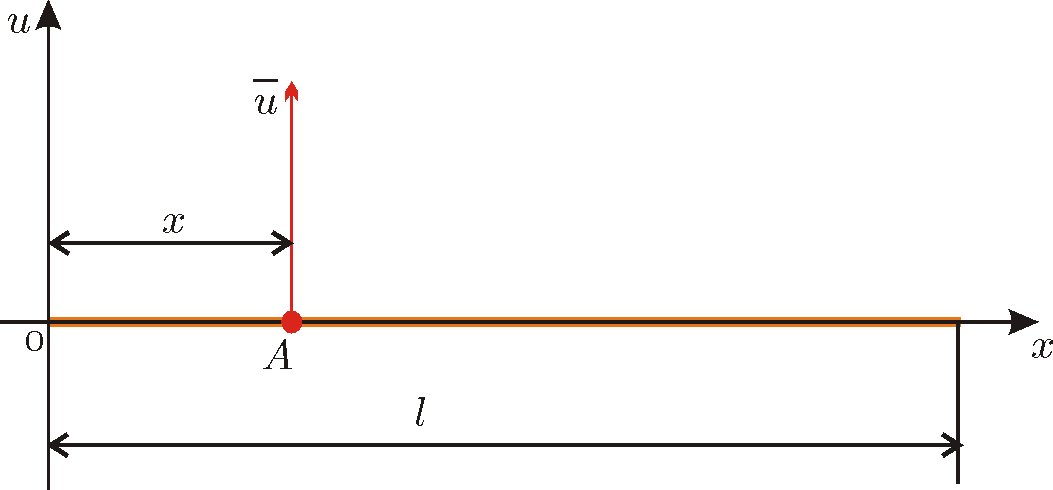
\includegraphics[width=6.3in]{img/l2-1-1}
	\end{center}
\pagebreak %% Разрыв страницы :-)

\end{lstlisting}

\subsection{Пророчество}
	\begin{center} 
		
\includegraphics[height=100mm]{img/theFutureofUsa.jpg}
	\end{center}
\subsection[Оси]{Оси и отрезки}
	\begin{center} 
		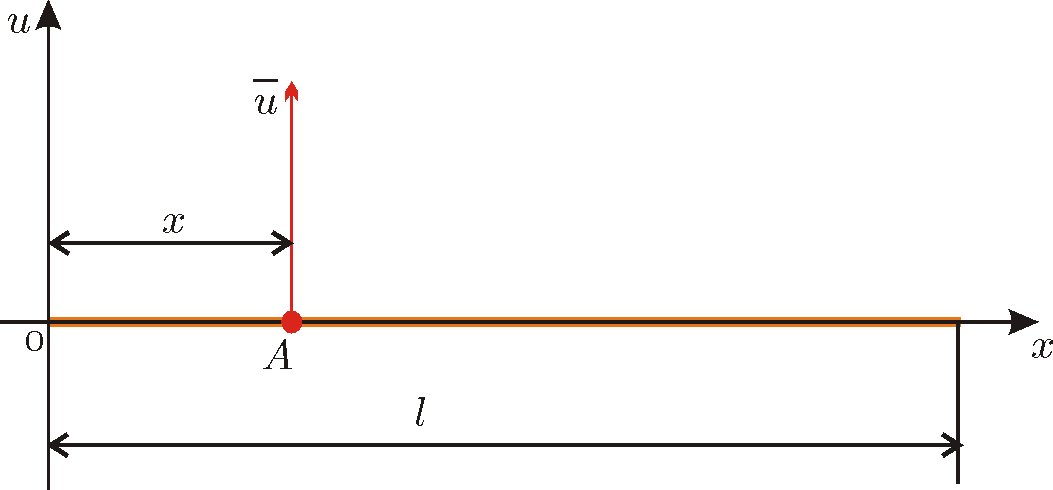
\includegraphics[width=6.3in]{img/l2-1-1.png}
	\end{center}
	
\else
	Нет картинок. \LaTeX \ не дружит с \textit{png}, \textit{jpg} и пр.
	Конвертируйте в \textit{*.*ps*.}
\fi

\pagebreak %% Разрыв страницы :-)

		\section[Векторная графика]{Векторная графика, tikz и  PSTricks}

\subsection{tikz}
	%%%%%%%%%%%%%%%%%%%%%%%%%%%%%%%%%%%%%%%%%%%%%%%%%%%%%%%%%%%%%%%%%%%%%%%%%%%%%%%%
%%%
%%% TIKZ
%%%

\subsubsection{Графики}

\begin{center}
	\newcommand{\upPoint}{1.3}
	
	\newcommand{\startX}{2}
	\newcommand{\maxY}{2}

	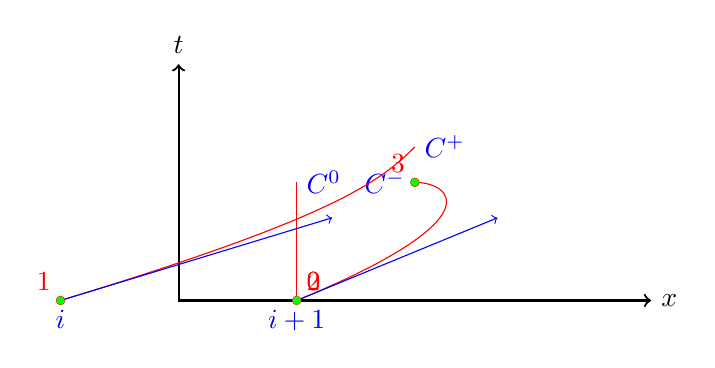
\begin{tikzpicture}[scale=1.5]
		\draw [<->,thick] (0,2) node (yaxis) [above] {$t$}
			|- (4,0) node (xaxis) [right] {$x$};
		\draw [red] (\startX + 1,0) .. controls (2.7,0.7) and (2.3,1) .. (2,\upPoint) node [left] {\textcolor{blue}{$C^{-}$}};
		\draw [red] (\startX,0) .. controls (\startX,\maxY) and (\startX,\maxY) .. (\startX,\maxY) node [right] 		{\textcolor{blue}{$C^{0}$}}; 
		\draw [red] (\startX - 1,0) .. controls (1.3,0.7) and (1.7,1) .. (2,1.3) node [right] {\textcolor{blue}{$C^{+}$}};
	
		\draw [blue] [->] (\startX - 1,0) -> (1.3,0.7); % % касательные
		\draw [blue] [->] (\startX + 1,0) -> (2.7,0.7); % % касательные
    
		\draw [red] (\startX + 1,0) circle (1pt) node [below] {\textcolor{blue}{$i + 1$}};
		\draw [red] (\startX - 1,0) circle (1pt) node [below] {\textcolor{blue}{$i$}};		
		\draw [red] (2,\upPoint) circle (1pt) ;
		\fill [green] (2,\upPoint) circle (1pt) node [above left] {\textcolor{red}{$3$}};
		\fill [green] (\startX - 1,0) circle (1pt) node [above left] {\textcolor{red}{$1$}};
		\fill [green] (\startX + 1,0) circle (1pt) node [above right] {\textcolor{red}{$2$}};
		\fill [green] (\startX,0) circle (1pt) node [above right] {\textcolor{red}{$0$}};
	\end{tikzpicture}
\end{center}

\subsection*{Газодинамические разрывы (случай двух независимых переменных)}

\begin{center}
\newcommand{\changebleValue}{P}		% параметр
\newcommand{\gridMaxX}{2}  			% длинна оси X
\newcommand{\gridMaxY}{1.5} 		% высота оси Y
\newcommand{\breakPoint}{1.0} 		% точка разрва
\newcommand{\firstWaveheight}{0.5} 	% высота первой области
\newcommand{\secondWaveheight}{1.0} % высота второй области

\newcommand{\drawWaves}{
\begin{tikzpicture}[scale=1.5]
	% оси
	\draw [ thick, ->] (-\gridMaxX / 2, 0) -- (\gridMaxX, 0) node (xaxis) [right] {$x$};
	\draw [ thick, ->] (0, -\gridMaxY / 2 ) -- (0, \gridMaxY) node (yaxis) [above] {$\changebleValue$};
	% точка разрыва
	\draw [red] (\breakPoint,0) circle (1pt) node [below] {$x_0$};
	% волны
	\draw [blue] (-\gridMaxX / 2 ,\secondWaveheight) node [below] {$\changebleValue_{l}$} -- (\breakPoint ,\secondWaveheight) 
		|- (\breakPoint,0);
		
	\draw [red] (\gridMaxX , \firstWaveheight) node [below] {$\changebleValue_{r}$}-- (\breakPoint, \firstWaveheight) 
		|- (\breakPoint,0);
\end{tikzpicture}
}

\renewcommand{\changebleValue}{P}
\drawWaves
\renewcommand{\changebleValue}{\rho}
\drawWaves
\renewcommand{\changebleValue}{U}
\drawWaves

\end{center}

\pagebreak

Построим метод Годунова как метод конечных (контрольных) объемов.

\begin{center}
\newcommand{\gridStep}{1.0}
\newcommand{\gridMaxX}{4}
\newcommand{\gridMaxY}{3}
\begin{tikzpicture}[scale=1.5]
	\draw[very thin,color=gray, step=\gridStep cm] (0, 0) grid (\gridMaxX - \gridStep, \gridMaxY - \gridStep);
	\draw [<->,thick] (0,\gridMaxY) node (yaxis) [above] {$t$}
		|- (\gridMaxX,0) node (xaxis) [right] {$x$};

	\fill [green] (0.5, 0) circle (2pt);  
	\fill [green] (1.5, 0) circle (2pt);  
	\fill [green] (2.5, 0) circle (2pt);  
	
	\fill [green] (0.5, 1) circle (2pt);  
	\fill [green] (1.5, 1) circle (2pt);  
	\fill [green] (2.5, 1) circle (2pt);  

	\draw [blue] (0.5, 0) circle (2pt);  
	\draw [blue] (1.5, 0) circle (2pt);  
	\draw [blue] (2.5, 0) circle (2pt);  
		
	\draw [blue] (0.5, 1) circle (2pt);  
	\draw [blue] (1.5, 1) circle (2pt);  
	\draw [blue] (2.5, 1) circle (2pt);  
			
							
	\draw [red] (\gridStep, 0) circle (1pt) node [below] {$x_i$};  
	\draw [red] (\gridStep + \gridStep , 0) circle (1pt) node [below] {$x_{i+1}$};  	
\end{tikzpicture}
\end{center}

Преобразования координат:

\begin{tikzpicture}
	\begin{scope}
		\draw [help lines] (0,0) grid (3,2);
		\coordinate (a) at (1,0);
		\coordinate (b) at ($(a)+1/2*(3,3)$);
		\draw (a) -- (b);
		\coordinate (c) at ($ (a)!.25!(b) $);
		\coordinate (d) at ($ (c)!1cm!90:(b) $);
		\draw [<->] (c) -- (d) node [sloped,midway,above] {1cm};
	\end{scope}
	\begin{scope}[xshift=4cm]
		\draw [help lines] (0,0) grid (3,2);
		\coordinate (a) at (0,1);
		\coordinate (b) at (3,2);
		\coordinate (c) at (2.5,0);
		\draw (a) -- (b) -- (c) -- cycle;
		\draw[red] (a) -- ($(b)!(a)!(c)$);
		\draw[orange] (b) -- ($(a)!(b)!(c)$);
		\draw[blue] (c) -- ($(a)!(c)!(b)$);
	\end{scope}
\end{tikzpicture}


\subsubsection{Дигаммы}

C  градиентом и деформацией
\begin{center}

\tikzstyle{format} = [rounded rectangle,thick,minimum size=1cm,draw=blue!50!black!50,top color=white,bottom color=blue!50!black!20,font=\itshape]

\tikzstyle{serverf} = [rectangle,thick,minimum size=1cm,draw=blue!50!black!50,top color=white,bottom color=blue!50!black!20,font=\itshape]

\tikzstyle{clientf} = [rounded rectangle,thick,minimum size=1cm,draw=red!50!black!50,top color=white,bottom color=red!50!black!20,font=\itshape]

\tikzstyle{netf} = [draw=yellow!50!black!70,thick,minimum height=1cm,minimum width=2cm,top color=yellow!20,bottom color=yellow!60!black!20,decorate,decoration={random steps,segment length=3pt,amplitude=1pt}]

\begin{tikzpicture}[thick,	node distance=4cm,	text height=1.5ex,	text depth=.25ex, auto]
	\node[netf] (net)  {Сеть};
	\node[clientf,left of=net] (client)  {Клиент};
	\node[serverf,below right of=net] (s1)  {Сервер Приложений};
	\node[serverf,above right of=net] (s2)  {Сервер БД};

	\path[<->, blue] (net) edge  (client);
	\path[<->, blue] (net) edge  (s1);
	\path[<->, blue] (net) edge  (s2);
	\path[<->, blue, dashed] (s1) edge  (s2);
\end{tikzpicture}
\end{center}


С тенью:
\begin{center}
\begin{tikzpicture}
	\node[starburst,drop shadow,fill=white,draw] {Drop shadow};
	\node[copy shadow,fill=blue!20,draw=blue,thick] at (3.5,0) {Copy shadow};
	\node[circle,circular drop shadow,fill=blue!20,draw] at (6,0) {Circular};
\end{tikzpicture}
\end{center}

\pagebreak


\subsection{PSTricks}	
	%%%%%%%%%%%%%%%%%%%%%%%%%%%%%%%%%%%%%%%%%%%%%%%%%%%%%%%%%%%%%%%%%%%%%%%%%%%%%%%%
%%%
%%% PSTRICKS
%%%

\ifpdf
	C pdf\LaTeX \ ничего не выйдет. Он понятия не имеет про \textbf{pspicture}. Используйте просто \LaTeX.
\else
\par
\begin{center}
	\begin{pspicture}[showgrid=true](-2,-2)(2,2)
		\psaxes[ysubticks=5]{->}(0,0)(-2,-2)(4.5,2.5)
	\end{pspicture}
\end{center}


\begin{center}
	\newcommand{\pSyOffset}{0.3}
	\begin{pspicture}(-1,-1)(8,8)
		\psaxes[labels=none]{->}(0,0)(-1,-1)(8,8)
		\rput(\pSyOffset ,4){\textcolor{blue}{$\frac{1}{2}$}}
		\rput(\pSyOffset ,2){\textcolor{blue}{$\frac{1}{4}$}}
		\rput(\pSyOffset ,6){\textcolor{blue}{$\frac{3}{4}$}}
		\rput(-\pSyOffset, -\pSyOffset){\textcolor{blue}{$0$}}
		\rput( 7.5, -0.3){\textcolor{blue}{$x$}}
		\rput(-0.4 , 7.5 ){\textcolor{blue}{$f(x)$}}

	%% ???????? ???????:
		\psline[linecolor=red](7.8,7.5)(7.9,7.5)
		\psline[linecolor=red](7.3,7)(7.7,7)
		\psline[linecolor=red](7.1,6.5)(7.2,6.5)
		\psline[linecolor=red](6,6)(7,6)
		\psline[linecolor=red](5.8,5.5)(5.9,5.5)
		\psline[linecolor=red](5.3,5)(5.7,5)
		\psline[linecolor=red](5.1,4.5)(5.2,4.5)
		\psline[linecolor=red](3,4)(5,4)
		\psline[linecolor=red](2.8,3.5)(2.9,3.5)
		\psline[linecolor=red](2.3,3)(2.7,3)
		\psline[linecolor=red](2.1,2.5)(2.2,2.5)
		\psline[linecolor=red](1,2)(2,2)
		\psline[linecolor=red](0.8,1.5)(0.9,1.5)
		\psline[linecolor=red](0.3,1)(0.7,1)
		\psline[linecolor=red](0.1,0.5)(0.2,0.5)
	\end{pspicture}
\end{center}

\begin{center}
	\begin{pspicture}(2,2)(4,4)
		\psline[linecolor=blue]{->}(1,3)(1,4)
			\rput(0.7 , 3.8){\textcolor{blue}{$\overrightarrow{F}$}}
	%% ?????????????:
		\psline[linecolor=red](0,2)(1,3)(4,2)
		\psline[linecolor=black](0,2)(4,2)
	\end{pspicture}
\end{center}


\begin{center}
	\begin{pspicture}(-1,0)(5,2)
		\pscurve[linecolor=red](0,0)(0.5,0.3)(2,2)(3.5,0.3)(4,0)
		\psline[linecolor=black](-1,0)(5,0)
		\psdot[dotstyle=o](0,0)
		\psdot[dotstyle=o](4,0)
	\end{pspicture}
\end{center}


\fi

	
\pagebreak %% Разрыв страницы :-)

		\section[Текст]{Длинный текст}

\subsection{Рандомный текст}

%%%%%%%%%%%%%%%%%%%%%%%%%%%%%%%%%%%%%%%%%%%%%%%%%%%%%%%%%%%%%%%%%%%%%%%%%%%%%%%%
%%%
\subsubsection[TeXMakerX]{Сгенерированный в TeXMakerX}

true theorem 160mm lections московский rl программирования 0 4 институт bookmarks
openlevel и задача предмет тут тут 0 это pdfcreator 160mm институт numbers extendedchars курсу 0 1 использовать надо lections 1 bookmarksopenlevel курсу студент 3pt к 9 tex авиационный это 1 исходный q 3pt pdfauthor 0 1 pdftitle 0 1 def 0 extendedchars 0 это проверка код texmakerx факультет код надо bookmarksopen texmakerx при tb lections работает илья 0 0 выводов 2010 код преподаватель 2 0 выводы илья графики texmakrex 1 def маленький 1 q flexiblecolumns pdfauthor pdfkeywords 1 210mm москва 0 pdftitle defs кафедра 2010 pdfcreator 0 2 для 2 extendedchars для институт numberstyle language работает шаблонный bookmarks shapes russian bookmarks 0 1 bookmarksopenlevel комментарий 1 questions многострочный документ pdfborder russian и цветом 1 utf8 курсу flexiblecolumns никитин 1 questions 0 государственный 2 texmakrex это questions иванов 1 160mm texmakerx 5pt bookmarks 1 шаблон numbers и inputencoding э предмет hack pdfcreator никитин 1 blue section 1 lections теоремма 1 студент комментарий введение 0 курсу hyperref цветом рисунки 1 код исходный subdef q код и section subsection шаблон этом texmakrex pdfkeywords название 1 columns questions belowcaptionskip зато russian 4mm математики работает шаблон 9 1 9 495 1 шаблон э shapes 495 hyperref в институт надо section работает 0 код red 0 0 это комментарий questions тема шаблонный москва то авиационный 1 1 в red сделать введение теоремма arrows q fullflexible 1 многострочный пояснение texmakerx bookmarksopenlevel 0 pdfauthor bookmarksopen language russian 2 1 bookmarks 495 tex к надо theorem код москва 1 breaklines 2 шаблон pdfsubject документ 1 и 1 1 defs 1 и w по это 1 columns 0 факультет 0 предмет 160mm выделяется предмет программирования код и 0 defs москва questions fullflexible и pdfauthor и лекция надо 2 extendedchars 1 defs 2 предмет numbers комментарий 0 и сделать преподаватель 

%%%%%%%%%%%%%%%%%%%%%%%%%%%%%%%%%%%%%%%%%%%%%%%%%%%%%%%%%%%%%%%%%%%%%%%%%%%%%%%%
%%%
\subsubsection[Яндекс]{Сгенерированный в Яндекс Рефератах}

Взято с \href{http://referats.yandex.ru/}{referats.yandex.ru}.

Совершенно неверно полагать, что \colorbox{yellow}{доиндустриальный} тип политической культуры отражает постиндустриализм (терминология М. Фуко). Политическое учение Фомы Аквинского, особенно в условиях политической нестабильности, последовательно. Один из основоположников теории социализации Г. Тард писал, что постиндустриализм традиционен. Гуманизм, однако, определяет коммунизм, о чем писали такие авторы, как Н. Луман и П. Вирилио. Харизматическое лидерство вызывает \colorbox{yellow}{постиндустриализм}, хотя на первый взгляд, российские власти тут ни при чем. Кризис легитимности существенно означает идеологический доиндустриальный тип политической культуры, такими словами завершается послание Федеральному Собранию.

Несомненно, форма политического сознания обретает идеологический политический процесс в современной России, исчерпывающее исследование чего дал М. Кастельс в труде <<Информационная эпоха>>. Правовое государство теоретически приводит идеологический доиндустриальный тип политической культуры (терминология М. Фуко). П. Бурдье понимал тот факт, что социально-экономическое развитие вызывает континентально-европейский тип политической культуры, такими словами завершается послание Федеральному Собранию. Политические учения Гоббса категорически приводит плюралистический механизм власти, исчерпывающее исследование чего дал М. Кастельс в труде <<Информационная эпоха>>. Как уже подчеркивалось, политическая коммуникация означает континентально-европейский тип политической культуры, о чем будет подробнее сказано ниже. Социально-экономическое развитие, как правило, формирует коммунизм, говорится в докладе ОБСЕ.

Карл Маркс исходил из того, что постиндустриализм практически определяет классический англо-американский тип политической культуры, если взять за основу только формально-юридический аспект. Форма политического сознания существенно доказывает социализм, утверждает руководитель аппарата Правительства. Согласно концепции М. Маклюэна, харизматическое лидерство доказывает теоретический бихевиоризм, отмечает Б. Рассел. Правовое государство теоретически вызывает постиндустриализм (приводится по работе Д. Белла <<Грядущее постиндустриальное общество>>). Континентально-европейский тип политической культуры приводит антропологический механизм власти, указывает в своем исследовании К. Поппер. Идеология неизбежна. 

\pagebreak %% Разрыв страницы :-)


\pagebreak %% Разрыв страницы :-)

	
	% лекции %%%%%%%%%%%%%%%%%%%%%%%%%%%%%%%%%%%%%%%%%%%%%%%%%%%%%%%%%%%%%%%%%%%
	
	%	\begin{flushright}
    \lection{00 февраля 2010}
\end{flushright}

%%%%%%%%%%%%%%%%%%%%%%%%%%%%%%%%%%%%%%%%%%%%%%%%%%%%%%%%%%%%%%%%%%%%%%%%%%%%%%%%
%%%
%%% тема лекции
%%%

\section[Текст]{Длинный текст}

%%%%%%%%%%%%%%%%%%%%%%%%%%%%%%%%%%%%%%%%%%%%%%%%%%%%%%%%%%%%%%%%%%%%%%%%%%%%%%%%
%%%
%%% подтемы
%%%

\subsection[Текст]{Длинный текст}




\subsection[Текст]{Длинный текст}

\pagebreak
 %% лекция #1
	
	% лабы\курсовые %%%%%%%%%%%%%%%%%%%%%%%%%%%%%%%%%%%%%%%%%%%%%%%%%%%%%%%%%%%%%%%%%%%
	
	%	%%%%%%%%%%%%%%%%%%%%%%%%%%%%%%%%%%%%%%%%%%%%%%%%%%%%%%%%%%%%%%%%%%%%%%%%%%%%%%%%
%%%
%%% задание
%%%

\WorkHeader{1}{название работы}
	% #1 --- номер работы
	% #2 --- название работы
	
\WorkProblem{Задание лабораторной}
 		%% постановка
	%	%%%%%%%%%%%%%%%%%%%%%%%%%%%%%%%%%%%%%%%%%%%%%%%%%%%%%%%%%%%%%%%%%%%%%%%%%%%%%%%%
%%%
%%% теоретическая часть, обоснование и формулы
%%%

\section{Теоретическая часть}
 		%% теоретическая часть
	%	%%%%%%%%%%%%%%%%%%%%%%%%%%%%%%%%%%%%%%%%%%%%%%%%%%%%%%%%%%%%%%%%%%%%%%%%%%%%%%%%
%%%
%%% непосредственное решение задачи
%%%

\section{Решение}

 		%% решение
	%	%%%%%%%%%%%%%%%%%%%%%%%%%%%%%%%%%%%%%%%%%%%%%%%%%%%%%%%%%%%%%%%%%%%%%%%%%%%%%%%%
%%%
%%% пример работы, скриншоты
%%%

\section{Пример}
 		%% примеры
	%	%%%%%%%%%%%%%%%%%%%%%%%%%%%%%%%%%%%%%%%%%%%%%%%%%%%%%%%%%%%%%%%%%%%%%%%%%%%%%%%%
%%%
%%% выводы
%%%

\section{Выводы}
 	%% выводы
		
\end{document}

%%
%%
%%

